%% mu -> e gamma

The current limit on the $\mu^+\to e^+ \gamma$ branching fraction is 
$5.7\times 10^{-13}$ at 90\% confidence level from MEG at 
PSI~\cite{Adam:2013mnn}, using 
$3.6\times 10^{14}$ stopped muons, from data taken in 2009--2011. 
Their sensitivity is dominated by 
accidental background, which is related to the muon stop rate
$R_\mu$ and various experimental resolutions~\cite{Baldini:2013ke}:
\begin{equation}
N_{\rm acc} \propto R_{\mu}^2 \times \Delta E_\gamma^2 \times \Delta P_e 
\times \Delta \Theta^2_{e\gamma} \times \Delta t_{e\gamma} \times T ,
%%{\rm Background} \propto \frac{R_\mu}{D} \Delta t_{e\gamma}
%%\frac{\Delta E_e}{m_\mu /2 } \left(\frac{\Delta E_\gamma}{15 m_\mu /2}\right )^2
%%\left(\frac{\Delta\theta_{e\gamma}}{2}\right)^2,
\end{equation}
where $\Delta t_{e\gamma}$, $\Delta P_e$, 
$\Delta E_\gamma$, and $\Delta\Theta_{e\gamma}$ are the resolutions of 
detector timing, positron momentum, photon energy, and positron-photon angle,
respectively, and $T$ is total data acquisition time. MEG will conitnue 
taking data through 2013. They expect to
approximately double their published dataset~\cite{G.Lim's talk at Argonne}.

The MEG upgrade plans to improve the experiment sensitivity by a factor of 10. 
They will increase the intensity of the surface beam, and use a thinner or
active stopping target. The detector upgrade includes a larger drift chamber with
thinner wires and smaller cells, an improved timing counter, and a larger LXe
calorimeter with SiPM readout. Data-taking is planned in the years 2016--2019.

The photon energy
resolution is a limiting factor in a $\mu^+\to e^+ \gamma$ search.  A pair spectrometer, based on reconstruction of $e^+e^-$ pair tracks produced in a
thin converter can provide improved photon energy resolution, at a sacrifice in efficiency. Even though only a small fraction of photons will convert,
the much higher power beam at Project X can
compensate for the loss of statistics~\cite{Fritz:2012aaa}. The thickness of the converter affects the energy 
resolution due to multiple scattering. Aa detailed study is thus required to prove that this approach does indeed provide an overall
improvement, as well as to optimize the converter thickness and to study the utility of making the converter active.

We have conducted an initial study of this concept using a fast simulation tool
(FastSim) originally developed for the Super$B$ experiment using the  \babar\ software
framework and analysis tools. FastSim allows us to model detector components
as two-dimensional shells of simple geometries. Particle scattering, energy
loss, secondary particle production (due to Compton scattering, Bremsstrahlung,
conversion, EM or hadron showers, {\it etc.}) are simulated at the intersection
of particles with detector shells. Tracks are reconstructed with a Kalman filter
into piece-wise trajectories. 

The FastSim model consists of a thin aluminum stopping target and a six-layer
cylindrical silicon detector. A 0.56 mm thick lead (10\%~$X_0$) half cylinder
covering 0--$\pi$ in azimuthal angle at $R=80$~mm serves as the photon converter. 
The target consists of two cones connected at their base; each cone is 30 mm 
high, 5 mm in radius, and 50~$\mu m$ thick.
Two silicon detector cylinders are placed close the target for better vertexing resolution;
two layers are placed just outside the Pb converter, and two layers a few cm away. The layout is shown in
Fig.~\ref{fig:muegamma-scheme}. The entire detector is placed in a 1~T
solenoidal magnetic field. 

\begin{figure}[htbp]
   \centering
   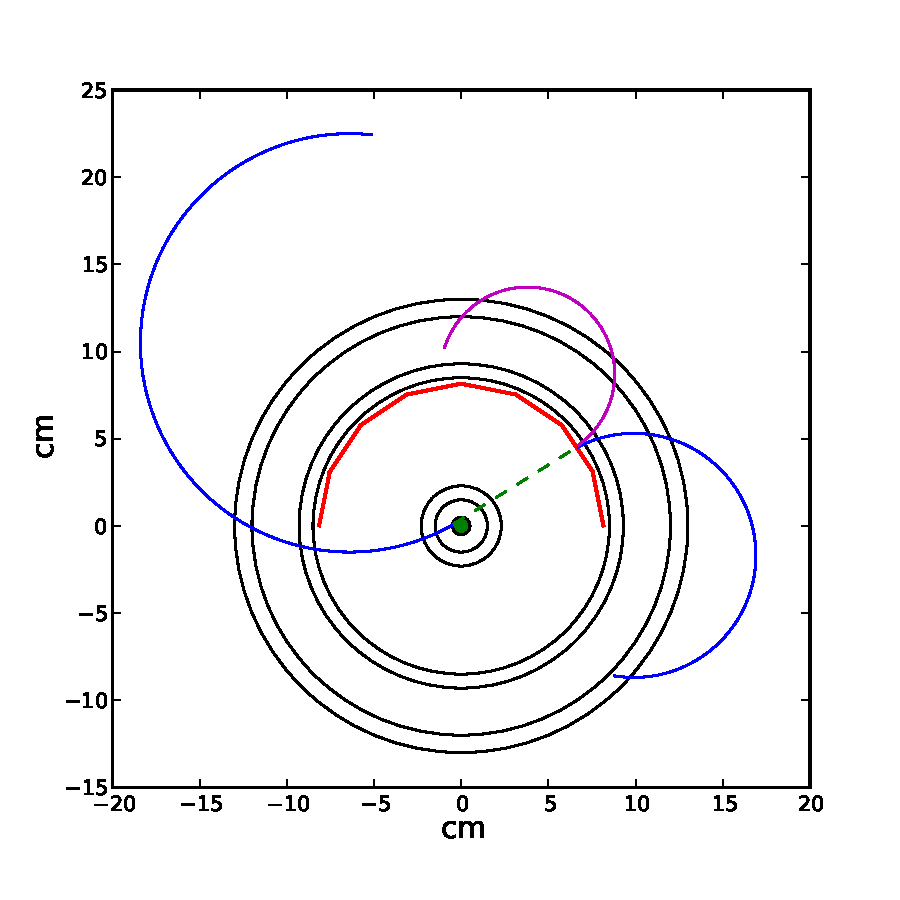
\includegraphics[width=0.5\textwidth]{ChargedLeptons/Figures/muegamma-schematic.pdf} 
   \caption{Schematic drawing (view transeverse to the muon beam axis) of the $\mu\to e\gamma$ detector used in the 
   FastSim model. }
   \label{fig:muegamma-scheme}
\end{figure}

We generate muons at rest and let them decay via $\mu^+\to e^+\gamma$ to study
the reconstruction efficiency and resolution. Approximately 1.3\% of generated
signal events are well-reconstructed, passing quality and fiducial selections criteria.
The photon energy resolution is approximately 200~keV, similar to the positron momentum
resolution, which corresponds to $0.37\%$ for 52.8~MeV photons. This is a great
improvement compared to the 1.7\%--2.4\% resolution of the current MEG and the  1.0\%--1.1\% resolution goal of the MEG
upgrade. The muon candidate mass resolution is 340~keV (85\% Gaussian core).
Figure~\ref{fig:muegamma-resolutions} shows the photon energy and muon candidate 
mass resolutions. The positron energy resolution is better than that of MEG, but not
as good as what is expected in the MEG upgrade. Angular resolution is similar to  the
current MEG.

\begin{figure}[htbp]
   \centering
   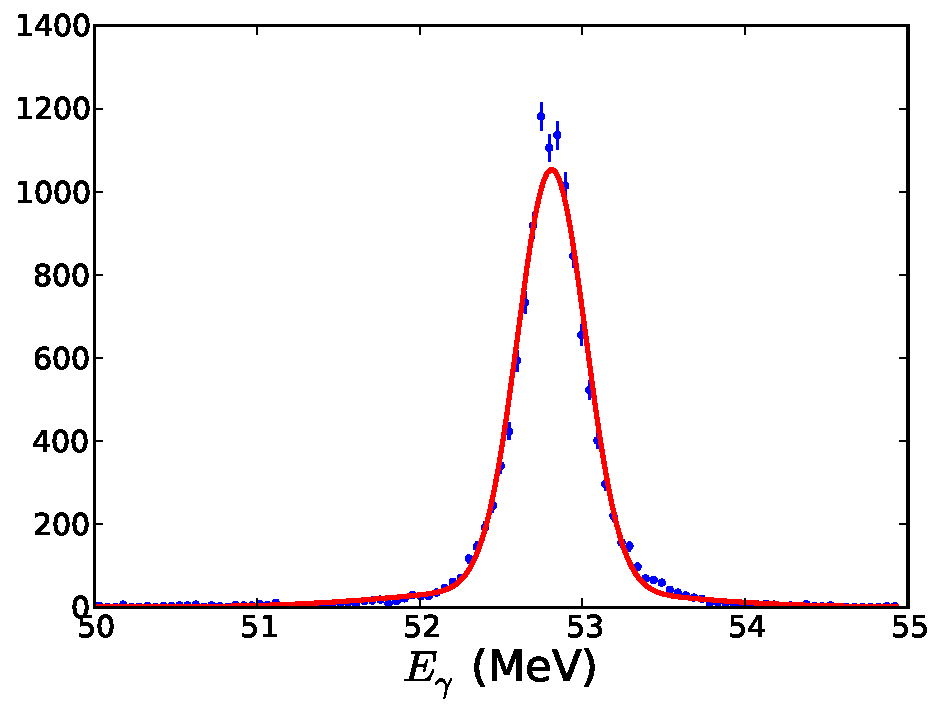
\includegraphics[width=0.48\textwidth]{ChargedLeptons/Figures/muegamma-gamma-resolution.pdf} 
   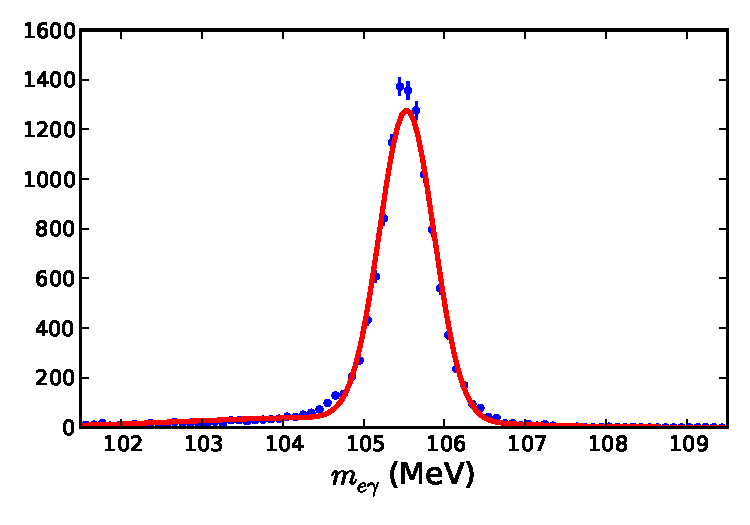
\includegraphics[width=0.48\textwidth]{ChargedLeptons/Figures/muegamma-mumass-resolution.pdf} 
   \caption{Photon energy and muon candidate mass resolutions in 
   $\mu^+\to e^+\gamma$ FastSim study. Fitted curve is a double-Gaussian 
   distribution.}
   \label{fig:muegamma-resolutions}
\end{figure}

Using a converted photon to increase the $\mu^+\to e^+\gamma$ detection sensitivity
thus appears to be a promising approach. Further studies are needed to quantify the requirements to improve upon the MEG upgrade sensitivity by an order of magnitude or more.

An alternative version of the photon conversion approach to a $\mu \to e \gamma$ experiment has also been discussed. In this version, consider a large volume solendoidal magnet, such as the KLOE coil, which has a radius of 2.9m, run at a field of perhaps 0.25T. A large volume, low mass cylindrical drift chamber provides many ($\ge$100) layers of tracking, utilizing small cells and having a total number of sense wires approaching $10^5$. Interspersed every ten layers is a 0.5 mm W converter shell. There are a sufficient number of points on the $e^+$ and $e^-$ tracks from converted photons behind each converter to reach a total conversion efficiency of perhaps 80\%, with excellent photon mass resolution. 




